\label{chapter_edmd}
In this third chapter, we introduce Extended Dynamic Mode Decomposition as a method for approximating eigenpairs from a dictionary of observables. In \Cref{section_resdmd} we introduce the problem of spectral pollution, and we explain how Residual DMD (ResDMD) can be used to remove it. Then we present pseudospectra as an effective method to individuate spectral pollution, as well as the use of ResDMD for approximating the pseudospectrum of the Koopman Operator. Finally, in \Cref{section_experiments} we reproduce some of he numerical examples presented in \cite{colbrook_rigorous_2021}.

\section{Extended Dynamic Mode Decomposition (EDMD)}
\label{section_edmd}
The \emph{Extended Dynamic Mode Decomposition} (EDMD), originally presented in \cite{williams_data-driven_2015}, is a method that seeks at approximating the Koopman Operator as a finite dimensional operator and then approximate the Koopman (eigenvalue, eigenfunction, mode) tuples from this finite dimensional approximation. The algorithm requires in input:
\begin{itemize}
    \item a dataset of snapshot pairs of the system state, $\{(\vb{x}_0^{(m)}, \vb{x}_1^{(m)})\}_{m = 1}^M$ with $\vb{x}_1^{(m)} = \vb{F}(\vb{x}_0^{(m)})$;
    \item a dictionary of observables $\mathcal{D} = \{\psi_1, \dots, \psi_K\} \subseteq \mathcal{D}(\mathcal{K})$. Let us define the vector-valued observable $\Psi:\Omega\to\C^{1\times K}$ as $\Psi(x) = [\psi_1(x), \dots, \psi_K(x)]$. The choice of the dictionary $\mathcal{D}$ is not easy and depends on the problem at hand. For the moment, let us assume that $\mathcal{D}$ is rich enough to approximate at least a few of the dominant Koopman eigenfunctions.
\end{itemize}

\subsection{Approximation of $\mathcal{K}$ and its eigenpairs}
Let $\phi\in\Span(\mathcal{D})$, then we can write:
\begin{equation*}
    \phi = \sum_{k=1}^K a_k\psi_k = \Psi\vb{a}, \qquad \vb{a}\in\C^K.
\end{equation*}
We aim at generating $\vb*{K}\in\C^{k\times k}$ finite dimensional approximation of $\mathcal{K}$ such that
\begin{equation}
    \label{k_finite_dimensional}
    \mathcal{K}\vb{\phi} = (\Psi \circ \vb{F})\vb{a} = \Psi\vb*K\vb{a} + r
\end{equation}
where the residual term $r = r(\vb{a}, \vb{x})$ is due to the fact that in general $\Span(\mathcal{D})$ is not $\mathcal{K}$-invariant. To obtain the "best" $\vb*{K}\in\C^{K\times K}$ it is natural to minimize the norm of the point-wise maximum of the residual of all possible $\phi\in\Span(\mathcal{D})$, i.e to solve the following problem \cite{colbrook_rigorous_2021}:
\begin{equation}
    \label{edmd_integral_problem}
    \argmin_{\vb*{K}\in\C^{K\times K}}\int_{\Omega} \max_{\vb{a}\in\C^k \\ \norm{\vb{a}} = 1}\abs{r(\vb{a}, \vb{x})}^2 d\omega(\vb{x}) = 
    \argmin_{\vb*{K}\in\C^{K\times K}}\int_{\Omega} \norm{\Psi(\vb{F}(\vb{x})) - \Psi(\vb{x})\vb*{K}}^2 d\omega(\vb{x}).
\end{equation}

We cannot directly compute the integral, thus we need to use a quadrature rule. We take as quadrature nodes our snapshot data $\{\vb{x}_0^{(m)}\}_{m = 1}^M$ with weights $\{w_m\}_{m = 1}^M$. The discretized problem reads:
\begin{equation}
\label{edmd_discretized_problem}
\begin{split}
    &\argmin_{\vb*{K}\in\C^{k\times k}} \sum_{j=1}^M w_j \norm{\Psi(\vb{F}(\vb{x}_0^{(j)})) - \Psi(\vb{x}_0^{(j)})\vb*{K}}^2 = \\
    = &\argmin_{\vb*{K}\in\C^{k\times k}} \sum_{j=1}^M w_j \norm{\Psi(\vb{x}_1^{(j)}) - \Psi(\vb{x}_0^{(j)})\vb*{K}}^2.
\end{split}    
\end{equation}
If we define the matrices
\begin{align}
\label{w_def}
\vb*{W} = \diag(w_1,\dots,w_M)\in\R_+^{M\times M} \\
\label{psi0_def}
\Psi_0 = \left[\Psi(\vb{x}_0^{(1)})^T,\dots,\Psi(\vb{x}_0^{(M)})^T\right]^T\in\C^{M\times K} \\
\label{psi1_def}
\Psi_1 = \left[\Psi(\vb{x}_1^{(1)})^T,\dots,\Psi(\vb{x}_1^{(M)})^T\right]^T\in\C^{M\times K}
\end{align}
we can write the weighted least-square problem in \eqref{edmd_discretized_problem} as 
\begin{equation}
    \label{edmd_discretized_problem_matrix}
    \argmin_{\vb*{K}\in\C^{k\times k}}\norm{\sqrt{\vb*{W}}(\Psi_1 - \Psi_0\vb*{K})}_F^2.
\end{equation}
The solution of the weighted least squares problem is
\begin{equation}
    \label{discretized_problem_solution}
    (\Psi_0^*\vb*{W}\Psi_0)\vb*{K} = \Psi_0^*\vb*{W}\Psi_1 \,\,\Longrightarrow\,\, \vb*{K} = (\Psi_0^*\vb*{W}\Psi_0)^{\dagger}(\Psi_0^*\vb*{W}\Psi_1),
\end{equation}
where by $\Longrightarrow$ we mean that $\vb*{K}$ is the solution with minimal norm, but to have uniqueness of the solution one might use regularization techniques. If the weights are the same for all quadrature points, then $\vb{K} = (\Psi_0^*\Psi_0)^{\dagger} \Psi_0^*\Psi_1 = \Psi_0^{\dagger}\Psi_1$ and we are back to the transpose of the matrix that we would obtain applying the DMD algorithm with vector-valued observable $\Psi^T$.

Observe that the matrices involved in the computations are
\begin{equation*}
    \label{psi_rewriting}
    \begin{split}
        \Psi_0^*\vb*{W}\Psi_0 & = \sum_{j=1}^M w_j \Psi(\vb{x}_0^{(j)})^* \Psi(\vb{x}_0^{(j)})\\
        \Psi_0^*\vb*{W}\Psi_1 & = \sum_{j=1}^M w_j \Psi(\vb{x}_0^{(j)})^* \Psi(\vb{x}_1^{(j)}).
    \end{split}
\end{equation*}
This rewriting is particularly advantageous when the number of snapshots is much larger than the size of the dictionary, i.e. $M >> K$, because each term of the sum can be computed individually and the products in \eqref{psi_rewriting} can be built iteratively, without the need of explicitly storing the matrices $\Psi_0,\,\Psi_1\in\C^{M\times K}$.

To approximate the eigenvalue-eigenfunction pair of the Koopman Operator, we use the eigenpairs of its finite dimensional approximation $\vb*{K}$. If $\lambda_j$ is an eigenvalue of $\vb*{K}$ with eigenvector $\bm{\xi}_j$, an approximation of an eigenvalue-eigenfunction pair of $\mathcal{K}$ is $(\lambda_j, \phi_j = \Psi\bm{\xi}_j)$.

A few final remarks for practical implementation of EDMD:
\begin{itemize}
    \item by reducing the size of the dictionary, we may assume without loss of generality that the matrix $(\Psi_0^*\vb*{W}\Psi_0)$ is non-singular. However, we might also consider using TSVD when computing its pseudo-inverse in practice.  
    \item Instead of computing the matrix $\vb*{K} = (\Psi_0^*\vb*{W}\Psi_0)^{\dagger}(\Psi_0^*\vb*{W}\Psi_1)$ and then its eigenpairs, it is often numerically more stable to solve the generalized eigenvalue problem $(\Psi_0^*\vb*{W}\Psi_0)\bm{\xi} = \lambda(\Psi_0^*\vb*{W}\Psi_1)\bm{\xi}$.
\end{itemize}

\subsection{Approximation of the Koopman modes for the full state observable}
Let us consider the full state observable
\begin{equation}
    \label{full_state_def}
    \vb{g}(\vb{x}) = 
    \begin{bmatrix}
    g_1(\vb{x}) \\
    \vdots \\
    g_d(\vb{x})
    \end{bmatrix} = 
    \begin{bmatrix}
    \vb{e}_1^*\vb{x} \\
    \vdots \\
    \vb{e}_d^*\vb{x}
    \end{bmatrix} = \vb{x}.
\end{equation}
Let us assume that $g_i\in\Span(\mathcal{D})$ for all $i = 1,\dots,d$. If this is not the case an intermediate step to project $g_i$ onto $\Span(\mathcal{D})$ is required, with the accuracy strongly depending on the choice of the dictionary. If $g_i\in\Span(\mathcal{D})$ we can write
\begin{equation}
    g_i = \sum_{k=1}^K b_{ki}\psi_k = \Psi\vb{b}_i
\end{equation}
and in matrix form
\begin{equation*}
    \vb{g} = \vb*{B}^T\Psi^T = (\Psi\vb*{B})^T, \qquad \vb*{B} = \left[\vb{b}_1, \dots,\vb{b}_d\right]\in\C^{k\times d}.
\end{equation*}
If we choose an orthonormal dictionary this step can be accomplished through the computation of the inner products $b_{ki} = \langle g_i, \psi_k \rangle$. This also accounts for the projection onto $\Span(\mathcal{D})$, if required.

Let $\bm{\Xi} = \left[\bm{\xi}_1,\dots,\bm{\xi}_K\right]$ be the matrix of the eigenvectors of $\vb*{K}$, the vector of approximate Koopman eigenfunctions $\Phi(\vb{x}) = \left[\phi_1(\vb{x}), \dots, \phi_K(\vb{x})\right]$ can be written as $\Phi = \Psi\bm{\Xi}$. Thus
\begin{equation}
    \vb{g} = \vb*{B}^T\Psi^T = \vb*{B}^T(\bm{\Xi}^T)^{-1}\Phi^T = (\bm{\Xi}^{-1}\vb*{B})^T\Phi^T.
\end{equation}
Since $\bm{\Xi}$ is the matrix of the eigenvectors of $\vb*{K}$, its inverse is $\bm{\Xi}^{-1} = \left[\vb{u}_1, \dots, \vb{u}_K\right]$ where $\vb{u}_i$ is the left eigenvector of $\vb*{K}$ also associated with $\lambda_i$ and appropriately scaled so that $\vb{u}_i^*\bm{\xi}_j = \delta_{ij}$. We can therefore compute the left eigenvectors of $\vb*{K}$ and letting  $\vb*{V} = (\vb*{U}^*\vb*{B})^T$, then
\begin{equation}
    \vb{g} = \vb*{V}\Psi^T = \sum_{k=1}^K \vb{v}_k\psi_k,
\end{equation}
i.e. $\vb{v}_j = (\vb{u}_j^*\vb*{B})^T$ is the $j$-th Koopman mode.

In conclusion, as summarized in \Cref{alg_edmd},  once we have computed the finite-dimensional approximation $\vb*{K}$ of the Koopman Operator:
\begin{itemize}
    \item the eigenvalues of $\vb*{K}$ are the EDMD approximation of the Koopman eigenvalues;
    \item the right eigenvectors of $\vb*{K}$ generate the approximation of the eigenfunctions;
    \item the left eigenvectors of $\vb*{K}$ generate the approximation of the Koopman modes.
\end{itemize}
If we are interested in an approximation of only a leading subset of eigenvalues, instead of a complete eigendecomposition of the matrix $\vb*{K}$ Krylov methods or other iterative methods might be considered to efficiently compute only the leading eigenpairs of $\vb*{K}$.

\begin{algorithm}
\caption{\textbf{: Extended Dynamic Mode Decomposition (EDMD)}}
\label{alg_edmd}
\textbf{Input}: Snapshot pairs of the system state, $\{(\vb{x}_0^{(m)}, \vb{x}_1^{(m)})\}_{m = 1}^M$, quadrature weights $\{w_m\}_{m = 1}^M$, dictionary of observables $\mathcal{D} = \{\psi_1, \dots, \psi_K\} \subseteq \mathcal{D}(\mathcal{K})$
\begin{algorithmic}[1]
\State Define the matrices $\vb*{W}$ \eqref{w_def}, $\Psi_0$ \eqref{psi0_def}, $\Psi_1$ \eqref{psi1_def}. 
\State Compute the matrices $(\Psi_0^*\vb*{W}\Psi_0)$ and $(\Psi_0^*\vb*{W}\Psi_1)$ .
\State Solve the generalized eigenvalue problem $(\Psi_0^*\vb*{W}\Psi_0)\bm{\xi} = \lambda(\Psi_0^*\vb*{W}\Psi_1)\bm{\xi}$.
\State Obtain the eigenfunctions as $\Phi = \Psi\bm{\Xi}$.
\If{want to compute eigenmodes}
    \State Write the (projection onto $\Span(\mathcal{D})$ of the) full observable $\vb{g}$ as $\vb{g} = \vb*{B}^T\Psi^T$.
    \State Compute the left eigenvectors $\vb{u}_j$ of $\vb*{K} = (\Psi_0^*\vb*{W}\Psi_0)^{\dagger}(\Psi_0^*\vb*{W}\Psi_1)$.
    \State Compute $\vb*{V} = (\vb*{U}^*\vb*{B})^T$, i.e $\vb{v}_j = (\vb{u}_j^*\vb*{B})^T$.
\EndIf
\end{algorithmic}
\textbf{Output:} Approximation of the Koopman eigenvalues ($\lambda_j$), eigenfunctions ($\phi_j$) and, possibly, eigemodes ($\vb{v}_j$).
\end{algorithm}


\section{Spectral pollution and Residual DMD (ResDMD)}
\label{section_resdmd}
To compute the eigenvalues of the Koopman Operator, we approximate the infinite-dimensional operator $\mathcal{K}$ by a finite matrix. Therefore, even if some of the eigenvalues produced by the EDMD algorithm are reliable, most of them are not. \emph{Pseudospectra} \cite{trefethen_spectra_2005} are a tool that allow us to detect this so called \emph{spectral pollution} \cite{colbrook_rigorous_2021}, i.e. spurious eigenvalues of the matrix $\vb*{K}$ that are only due to the discretization and have no connection with the latent Koopman Operator.

\begin{definition}[Pseudospectrum of a square matrix]
Given a matrix $\vb*{A}\in\C^{n\times n}$ and $\varepsilon > 0$, the $\varepsilon$-pseudospectrum of $\vb*{A}$ is defined as
\begin{equation}
    \label{pseudospectrum_matrix_def}
    \sigma_{\varepsilon}(\vb*{A}) = \left\{ \lambda\in\C \text{ : } \norm{(\vb*{A} - \lambda \vb*{I})^{-1}}_2 \geq \frac{1}{\varepsilon}\right\} = \left\{ \lambda\in\C \text{ : } \sigma_{\mathrm{min}}(\vb*{A} - \lambda \vb*{I}) \leq \varepsilon \right\} %\bigcup_{\norm{\vb*{B}} \leq \varepsilon} \sigma(\vb*{A}+ \vb*{B}),
\end{equation}
where $\sigma_{\mathrm{min}}(\vb*{M})$ indicates the minimum singular value of the matrix $\vb*{M}$.
\end{definition}
In analogy with the second form of previous definition, we can define the pseudospectrum of a rectangular matrix pencil as follows.
\begin{definition}[Pseudospectrum of a rectangular matrix pencil]
Given two rectangular matrices $\vb*{A},\vb*{B} \in\C^{m\times n}$ and $\varepsilon > 0$, the $\varepsilon$-pseudospectrum of the matrix pencil $\vb*{A}- \lambda \vb*{B}$ is defined as
\begin{equation}
    \label{pseudospectrum_matrix_pencil_def}
    \sigma_{\varepsilon}(\vb*{A}, \vb*{B}) = \left\{ \lambda\in\C \text{ : } \sigma_{\mathrm{min}}(\vb*{A} - \lambda \vb*{B}) \leq \varepsilon \right\} %\bigcup_{\norm{\vb*{B}} \leq \varepsilon} \sigma(\vb*{A}+ \vb*{B}),
\end{equation}
The pseudospectrum of a rectangular matrix $\vb*{A}\in\C^{m\times n}$ is defined as $    \sigma_{\varepsilon}(\vb*{A}, \vb*{I})$ where
\begin{equation}
    \vb*{I} = \begin{bmatrix} \vb*{I}_n \\ \vb*{0}_{m-n,n}\end{bmatrix} \text{ if $n<m$}, \qquad \vb*{I} = \begin{bmatrix} \vb*{I}_m & \vb*{0}_{m,n-m}\end{bmatrix} \text{ if $m<n$}.
\end{equation}
\end{definition}
However, $\mathcal{K}$ is an infinite dimensional operator and might be unbounded, hence following \cite{colbrook_rigorous_2021} we can define
\begin{equation}
    \label{pseudospectrum_koopman_def}
    \sigma_{\varepsilon}(\mathcal{K}) = \mathrm{cl}\left( \left\{ \lambda\in\C \text{ : } \norm{(\mathcal{K} - \lambda \cdot \mathrm{id})^{-1}} > \frac{1}{\varepsilon}\right\} \right) = \mathrm{cl}\left( \bigcup_{\norm{\vb*{B}} < \varepsilon} \sigma(\mathcal{K}+ \vb*{B}) \right)
\end{equation}
where $\mathrm{id}$ is the identity operator and $\mathrm{cl}$ is the closure of a set.



\subsection{ResDMD to remove spectral pollution}
The \emph{Residual DMD} (ResDMD) algorithm performs the same steps of EDMD, but then discards the approximate eigenpairs $\{(\lambda_j,\, \phi_j)\}_j$ that have a residual above a certain prescribed tolerance $\varepsilon$. Given a candidate eigenpair $(\lambda, \phi)$ of $\mathcal{K}$, where $\phi = \Psi\bm{\xi}$, to measure its accuracy we can consider the relative residual
\begin{equation}
    \label{residual_definiton}
    \begin{split}
        &\mathrm{res}(\lambda, \phi)^2 = \frac{\int_{\Omega} \abs{[\mathcal{K}\phi](x) - \lambda\phi(x)}^2\,\,d\omega(x)}{\int_{\Omega} \abs{\phi(x)}^2\,\,d\omega(x)} 
        = \frac{\langle (\mathcal{K} - \lambda \cdot\mathrm{id})\phi, (\mathcal{K} - \lambda \cdot \mathrm{id})\phi \rangle}{\langle\phi , \phi \rangle} = \\
        & = \frac{\sum_{j,k = 1}^K \overline{\xi}_j\xi_k \left( \langle\mathcal{K}\psi_k, \mathcal{K}\psi_j\rangle - \lambda \langle\psi_k, \mathcal{K}\psi_j\rangle - \overline{\lambda}\langle\mathcal{K}\psi_k, \psi_j\rangle + \abs{\lambda}^2 \langle\psi_k, \psi_j\rangle\right)}{\sum_{j,k = 1}^K \overline{\xi}_j\xi_k \langle\psi_k, \psi_j\rangle}.
    \end{split}
\end{equation}
Once again, this integral cannot be computed exactly and to approximate it we use the same quadrature rule used to approximate \eqref{edmd_integral_problem}. Hence:
\begin{equation}
    \label{residual_approx}
    \begin{split}
        \mathrm{res}(\lambda, \phi)^2 &\approx \frac{\sum_{j,k = 1}^K \overline{\xi}_j\xi_k \left( (\Psi_1^*\vb*{W}\Psi_1)_{jk} - \lambda (\Psi_1^*\vb*{W}\Psi_0)_{jk} - \overline{\lambda}(\Psi_0^*\vb*{W}\Psi_1)_{jk} + \abs{\lambda}^2 (\Psi_0^*\vb*{W}\Psi_0)_{jk}\right)}{\sum_{j,k = 1}^K \overline{\xi}_j\xi_k (\Psi_0^*\vb*{W}\Psi_0)_{jk}} = \\ 
        & = \frac{\bm{\xi}^* \left((\Psi_1^*\vb*{W}\Psi_1) - \lambda (\Psi_1^*\vb*{W}\Psi_0) - \overline{\lambda}(\Psi_0^*\vb*{W}\Psi_1) + \abs{\lambda}^2 (\Psi_0^*\vb*{W}\Psi_0)\right) \bm{\xi}}{\bm{\xi}^*(\Psi_0^*\vb*{W}\Psi_0)\bm{\xi}} =: \widetilde{\mathrm{res}}^2(\lambda, \phi).
    \end{split}
\end{equation}
If $\widetilde{\mathrm{res}}(\lambda, \phi) > \varepsilon$, the eigenpair $(\lambda, \phi)$ is discarded. This algorithm is summarized in \Cref{alg_resdmd}. Observe that to compute the approximation of the residual we only need to compute $(\Psi_1^*\vb*{W}\Psi_1)$, because the other matrices are already computed in the standard EDMD algorithm. 

\begin{algorithm}
\caption{\textbf{: Residual Dynamic Mode Decomposition (ResDMD)}}
\label{alg_resdmd}
\textbf{Input}: Snapshot pairs of the system state, $\{(\vb{x}_0^{(m)}, \vb{x}_1^{(m)})\}_{m = 1}^M$, quadrature weights $\{w_m\}_{m = 1}^M$, dictionary of observables $\mathcal{D} = \{\psi_1, \dots, \psi_K\} \subseteq \mathcal{D}(\mathcal{K})$, tolerance $\varepsilon > 0$.
\begin{algorithmic}[1]
\State Execute \Cref{alg_edmd}.
\State Compute the matrix $(\Psi_1^*\vb*{W}\Psi_1)$.
\For{each approximate eigenpair $(\lambda_j,\phi_j)$}
    \State Compute $\widetilde{\mathrm{res}}(\lambda_j, \phi)_j$ as in \eqref{residual_approx}.
    \If {$\widetilde{\mathrm{res}}(\lambda_j, \phi)_j \geq \varepsilon$}
        \State Discard the approximate eigenpair $(\lambda_j,\phi_j)$.
    \EndIf
\EndFor
\end{algorithmic}
\textbf{Output:} Approximation of the eigenvalues ($\lambda_j$), eigenfunctions ($\phi_j$) with $\widetilde{\mathrm{res}}(\lambda_j, \phi)_j < \varepsilon$
\end{algorithm}

The above-described cleanup procedure avoids spectral pollution and if the quadrature converges, in the large data limit, removes eigenpairs with a residual above the prescribed tolerance $\varepsilon$ and retains only eigenpairs that are inside the $\varepsilon$-pseudospectrum of $\mathcal{K}$. This is precised in the following proposition.
\begin{prop}[\cite{colbrook_rigorous_2021}, Theorem 4.1]
Assume that the quadrature rule converges, i.e. that
\begin{equation*}
    \lim_{M\to+\infty}(\Psi_0^*\vb*{W}\Psi_0)_{jk} = \langle \psi_j, \psi_k \rangle, \quad
    \lim_{M\to+\infty}(\Psi_0^*\vb*{W}\Psi_1)_{jk} = \langle \psi_j, \mathcal{K}\psi_k \rangle, \quad
    \lim_{M\to+\infty}(\Psi_1^*\vb*{W}\Psi_1)_{jk} = \langle \mathcal{K}\psi_j, \mathcal{K}\psi_k \rangle.
\end{equation*}
Let us denote by $\Lambda$ the eigenvalues in the output of \Cref{alg_resdmd}, then
\begin{equation}
    \limsup_{M\to+\infty} \max_{\lambda\in\Lambda}\norm{(\mathcal{K} - \lambda)^{-1}}^{-1} \leq \epsilon.
\end{equation}
\end{prop}

\subsection{ResDMD to approximate the pseudospectrum}
In spite of the fact that the eigenvalues returned by \Cref{alg_resdmd} lie in the $\varepsilon$-pseudospectrum (in the large data limit), the eigenvalues of $\vb*{K}$ might not approximate the whole spectrum of $\mathcal{K}$ and therefore it might not be possible to approximate the whole $\varepsilon$-pseudospectrum of $\mathcal{K}$ using \Cref{alg_resdmd}. A simple modification of \Cref{alg_resdmd} allows us to draw an approximation of the $\varepsilon$-pseudospectrum of $\mathcal{K}$ starting from a grid of points in the complex plane. Given a point $z_j\in\C$ on a grid, we search the function $\psi_j$ in $\Span(\mathcal{D})$ that minimizes $\mathrm{res}(z_j, \psi_j)$, i.e. we solve
\begin{equation}
    \label{grid_continuous}
    \tau_j = \min_{\vb{g}\in\C^K} \mathrm{res}(z_j, \Psi\vb{g}), \qquad \vb{g}_j = \argmin_{\vb{g}\in\C^K} \mathrm{res}(z_j, \Psi\vb{g}).
\end{equation}
Following \eqref{residual_approx}, the discretized problem reads:
\begin{equation}
    \label{grid_discretized}
    \tau_j = \min_{\vb{g}\in\C^K} \frac{\vb{g}^*\vb*{D}(z_j)\vb{g}}{\vb{g}^*(\Psi_0^*\vb*{W}\Psi_0)\vb{g}}\,\,, \qquad \vb{g}_j = \argmin_{\vb{g}\in\C^K} \frac{\vb{g}^*\vb*{D}(z_j)\vb{g}}{\vb{g}^*(\Psi_0^*\vb*{W}\Psi_0)\vb{g}}
\end{equation}
\begin{equation}
    \label{D(z)_definition}
    \begin{split}
        \vb*{D}(z_j) &= (\Psi_1^*\vb*{W}\Psi_1) - z_j (\Psi_1^*\vb*{W}\Psi_0) - \overline{z}_j(\Psi_0^*\vb*{W}\Psi_1) + \abs{z_j}^2 (\Psi_0^*\vb*{W}\Psi_0) =\\ 
        & = (\Psi_1 - z_j\Psi_0)^*\vb*{W}(\Psi_1 - z_j\Psi_0).
    \end{split}
\end{equation}
The matrices $(\Psi_0^*\vb*{W}\Psi_0)$ and $\vb*{D}(z_j)$ are hermitian positive semidefinite. If we also assume that $\Psi_0$ has full column rank, from the properties of the Rayleigh quotient solving \eqref{grid_discretized} is equivalent to finding the smallest eigenvalue and the associated eigenvector of the generalized eigenvalue problem $\vb*{D}(z_j)\vb{g} = \tau(\Psi_0^*\vb*{W}\Psi_0)\vb{g}$, which allows for a more efficient computation. This algorithm, proposed in \cite{colbrook_rigorous_2021}, is summarized in \Cref{alg_pseudospectrum}. Convergence guarantees for the approximation of the $\varepsilon$-pseudospectrum can be found in \cite{colbrook_rigorous_2021}.

\begin{algorithm}
\caption{\textbf{: ResDMD for pseudospectrum approximation}}
\label{alg_pseudospectrum}
\textbf{Input}: Snapshot pairs of the system state, $\{(\vb{x}_0^{(m)}, \vb{x}_1^{(m)})\}_{m = 1}^M$, quadrature weights $\{w_m\}_{m = 1}^M$, dictionary of observables $\mathcal{D} = \{\psi_1, \dots, \psi_K\} \subseteq \mathcal{D}(\mathcal{K})$, tolerance $\varepsilon > 0$, grid $z_1, \dots, z_k \in\C$.
\begin{algorithmic}[1]
\State Define the matrices $\vb*{W}$ \eqref{w_def}, $\Psi_0$ \eqref{psi0_def}, $\Psi_1$ \eqref{psi1_def}. 
\State Compute the matrices $(\Psi_0^*\vb*{W}\Psi_0)$, $(\Psi_0^*\vb*{W}\Psi_1)$ and $(\Psi_1^*\vb*{W}\Psi_1)$.
\For{each $z_j$ in the grid}
\State Solve $\tau_j = \min_{\vb{g}\in\C^K} \mathrm{res}(z_j, \Psi\vb{g}),\,\, \vb{g}_j = \argmin_{\vb{g}\in\C^K} \mathrm{res}(z_j, \Psi\vb{g})$.
\EndFor
\end{algorithmic}
\textbf{Output:} Estimate of the $\varepsilon$-pseudospectrum $\{z_j\,:\,\tau_j < \varepsilon\}$ and corresponding approximate eigenfunctions $\{\vb{g}_j\,:\,\tau_j < \varepsilon\}$. 
\end{algorithm}

The following proposition allows to rewrite the pseudospectrum approximation provided by \Cref{alg_pseudospectrum} as the pseudospectrum either of a rectangular matrix pencil or of a rectangular matrix.
\begin{prop}
\label{prop_pseudospectrum}
Let us assume that $\Psi_0$ has full column rank and let us consider the singular value decomposition $\sqrt{\vb*{W}}\Psi_0 = \vb*{U}\bm{\Sigma}\vb*{V}$, where $\vb*{U}\in\C^{M\times K}$ and $\bm{\Sigma},\vb*{V}\in\C^{K\times K}$. Then the approximation of the pseudospectrum of the Koopman operator provided by \Cref{alg_pseudospectrum} coincides with the pseudospectrum of the rectangular matrix pencil
\begin{equation}
    \sqrt{\vb*{W}}\Psi_1 \vb*{V}\bm{\Sigma}^{-1} - \lambda\vb*{U}.
\end{equation}
Moreover if the columns of $\vb*{U}_{\perp}$ complete the columns of $\vb*{U}$ to an orthonormal basis of $\C^{M}$, then the pseudospectrum approximation coincides also with the pseudospectrum of the rectangular matrix
\begin{equation}
    \begin{bmatrix}
    \vb*{U}^*\sqrt{\vb*{W}}\Psi_1 \vb*{V}\bm{\Sigma}^{-1}\\
    \vb*{U}_{\perp}^*\sqrt{\vb*{W}}\Psi_1 \vb*{V}\bm{\Sigma}^{-1}
    \end{bmatrix} = 
    \begin{bmatrix}
    \bm{\Sigma}\vb{V}^*(\Psi_0^\dagger \Psi_1)\vb{V}\bm{\Sigma}^{-1}\\
    \vb*{U}_{\perp}^*\sqrt{\vb*{W}}\Psi_1 \vb*{V}\bm{\Sigma}^{-1}
    \end{bmatrix}.
\end{equation}
\end{prop}
\begin{proof}
Let $z\in\C$ and let us consider the corresponding residual:
\begin{equation*}
\begin{split}
    \tau(z) &= \min_{\vb{g}\in\C^K} \frac{\vb{g}^*\vb*{D}(z)\vb{g}}{\vb{g}^*(\Psi_0^*\vb*{W}\Psi_0)\vb{g}} = \min_{\vb{g}\in\C^K} \frac{\vb{g}^*\vb*{D}(z)\vb{g}}{\vb{g}^*(\vb*{V}\bm{\Sigma}\vb*{V}^*)^2\vb{g}} =  \min_{\vb{v}\in\C^K} \frac{\vb{v}^*(\vb*{V}\bm{\Sigma}^{-1}\vb*{V}^*)\vb*{D}(z)(\vb*{V}\bm{\Sigma}^{-1}\vb*{V}^*)\vb{v}}{\vb{v}^*\vb{v}} = \\
    &= \lambda_{\min}\left((\vb*{V}\bm{\Sigma}^{-1}\vb*{V}^*)\vb*{D}(z)(\vb*{V}\bm{\Sigma}^{-1}\vb*{V}^*)\right) = \lambda_{\min}\left(\vb*{C}(z)^*\vb*{C}(z)\right) = \sigma_{\min}(\vb*{C}(z))^2
\end{split}
\end{equation*}
where from \eqref{D(z)_definition} we can write $\vb*{C}(z) = \sqrt{\vb*{W}}(\Psi_1 - z\Psi_0)\vb*{V}\bm{\Sigma}^{-1}\vb*{V}^*$. Hence $\tau(z) = \sigma_{\min}(\vb*{C}(z))^2 \leq \varepsilon^2$ if and only if $\sigma_{\min}(\vb*{C}(z)) \leq \varepsilon$. Now observe that
\begin{equation*}
    \begin{split}
        \sigma_{\min}(\vb*{C}(z)) &= \sigma_{\min}(\sqrt{\vb*{W}}(\Psi_1 - z\Psi_0)\vb*{V}\bm{\Sigma}^{-1}\vb*{V}^*) = \sigma_{\min}(\sqrt{\vb*{W}}(\Psi_1 - z\vb*{U}\bm{\Sigma}\vb*{V}^*)\vb*{V}\bm{\Sigma}^{-1}\vb*{V}^*) = \\
        &= \sigma_{\min}(\sqrt{\vb*{W}}(\Psi_1 - z\vb*{U}\bm{\Sigma}\vb*{V}^*)\vb*{V}\bm{\Sigma}^{-1}) = \sigma_{\min}(\sqrt{\vb*{W}}\Psi_1\vb*{V}\bm{\Sigma}^{-1} - z\vb*{U})
    \end{split}
\end{equation*}
from which follows the first statement. 

Moreover $\vb*{Q} = [\vb*{U}\,\lvert\,\vb*{U}_\perp]$ is an unitary matrix, hence multiplying by $Q$ on the left the singular values are preserved, yielding:
\begin{equation*}
    \begin{split}
        \sigma_{\min}(\vb*{C}(z)) &= \sigma_{\min}(\vb*{Q}^*\sqrt{\vb*{W}}\Psi_1\vb*{V}\bm{\Sigma}^{-1} - z\vb*{Q}^*\vb*{U}) = \\
        & = \sigma_{\min}\left( 
        \begin{bmatrix}
        \vb*{U}^*\sqrt{\vb*{W}}\Psi_1 \vb*{V}\bm{\Sigma}^{-1}\\
        \vb*{U}_{\perp}^*\sqrt{\vb*{W}}\Psi_1 \vb*{V}\bm{\Sigma}^{-1}
        \end{bmatrix} - z 
        \begin{bmatrix}
        \vb*{I}_K\\
        \vb*{0}_{M-K, K}\\
        \end{bmatrix}
        \right).
    \end{split}
\end{equation*}
Finally one can write the upper part of the matrix as:
\begin{equation*}
    \vb*{U}^*\sqrt{\vb*{W}}\Psi_1 \vb*{V}\bm{\Sigma}^{-1} = \bm{\Sigma} \vb*{V}^* \vb*{V}\bm{\Sigma}^{-1}\vb*{U}^*\sqrt{\vb*{W}}\Psi_1 \vb*{V}\bm{\Sigma}^{-1} = \bm{\Sigma}\vb{V}^*(\Psi_0^\dagger \Psi_1)\vb{V}\bm{\Sigma}^{-1}.
\end{equation*}
\end{proof}

From the previous rewriting, one can use standard techniques for the computation of pseudospectra of rectangular matrices \cite{wright_pseudospectra_2002}, as long as $M$ is not too big. Observe indeed that the matrix pencil in \Cref{prop_pseudospectrum} is of size $M\times K$, while the generalized eigenvalue problems in \Cref{alg_pseudospectrum} involve matrices of size $K\times K$.

\section{Numerical Examples}
\label{section_experiments}
In this section we reproduce two numerical examples from Section 4 of \cite{colbrook_rigorous_2021}.

\subsection{Gauss iterated map}
\label{sect_gauss_iterated_map}
The Gauss iterated map is a function $F:\R\to\R$ defined by $F(x) =\exp(\alpha x^2) + \beta $, where $\alpha$ and $\beta$ are parameters. We consider the case $\alpha = 2$ and $\beta = 1-\exp(-\alpha) = 1 - e^{-2}$, with state space $\Omega = [-1, 0]$ and the Lebesgue measure. Observe that with such a choice of the parameters, $F$ maps $\Omega$ onto itself, as necessary to have a well defined dynamical system on $\Omega$. As a dictionary of observable $\mathcal{D}$ we consider the first $K$ normalized Legendre polynomials transplanted to the interval $\Omega$. To understand the influence on the accuracy of the algorithm of the choice of the snapshot pairs $\{(\vb{x}_0^{(m)}, \vb{x}_1^{(m)})\}_{m = 1}^M$, which are the nodes of the quadrature rule, we consider four different types of quadrature rule:
\begin{itemize}
    \item Gauss-Legendre: $\{\vb{x}_0^{(m)}\}_{m = 1}^M$ are the Gauss-Legendre quadrature nodes transplanted to the interval $\Omega$, with $\{w_m\}_{m = 1}^M$ the corresponding quadrature weights.
    \item Trapezoidal: $\vb{x}_0^{(m)} = -1 + \frac{m-1}{M-1}$, with $w_m = \frac{1}{M-1},\,\,m = 2,\dots, M-1$ and $w_1 = w_M = \frac{1}{2(M-1)}$.
    \item Riemann sum: $\vb{x}_0^{(m)} = -1 + \frac{m-1}{M-1}$, with $w_m = \frac{1}{M-1},\,\,m = 1,\dots, M$.
    \item Montecarlo: $\{\vb{x}_0^{(m)}\}_{m = 1}^M$ are chosen uniformly at random in over the interval $\Omega$, with $w_m = \frac{1}{M-1},\,\,m = 1,\dots, M$. 
\end{itemize}

\Cref{fig_resdmd_quadrature_comparison} shows the approximations of the eigenvalues of the Koopman Operator computed using DMD, EDMD and ResDMD for each of the four quadrature rules. \Cref{gauss_pseudospectrum_convergence} shows the approximation of the $\varepsilon$-pseudospectrum for $\varepsilon = 0.3,\,0.1,\,0.01,\,0.001$ computed using \Cref{alg_pseudospectrum} and the convergence of the different quadrature rules measured as $\max_{1\leq j,k \leq K} \abs{(\Psi_0^* W \Psi_1)_{jk} - \langle\mathcal{K}\psi_k, \psi_j\rangle}$.

It can be seen that for the Montecarlo and the Riemann Sums quadrature rules, which use the same weights for all quadrature points, EDMD and DMD compute the same eigenvalues (magenta dots and green pluses overlap in \Cref{fig_resdmd_quadrature_comparison}). The outputs of the two algorithms are slightly dissimilar for the Trapezoidal rule, which changes the weights only at the extremes, while they significantly differ for the Gauss-Legendre rule.

The convergence rates are in agreement with standard theoretical results on numerical integration \cite{quarteroni_numerical_2007}, with the Gauss-Legendre quadrature converging exponentially and the other quadrature rules polynomially. It can be understood that if one has the possibility of choosing the initial condition of the snapshot data, selecting them wisely can make the discretized problem significantly closer to the continuous one. This has a strong impact also on the accuracy of the eigenvalues computed using \Cref{alg_resdmd}. Indeed, the more accurate is the computation of the residual's integral, the more eigenvalues can be removed due to a too high residual, as shown in \Cref{fig_resdmd_quadrature_comparison}.

\begin{figure}[h]
\centering
\makebox[\textwidth][c]{
    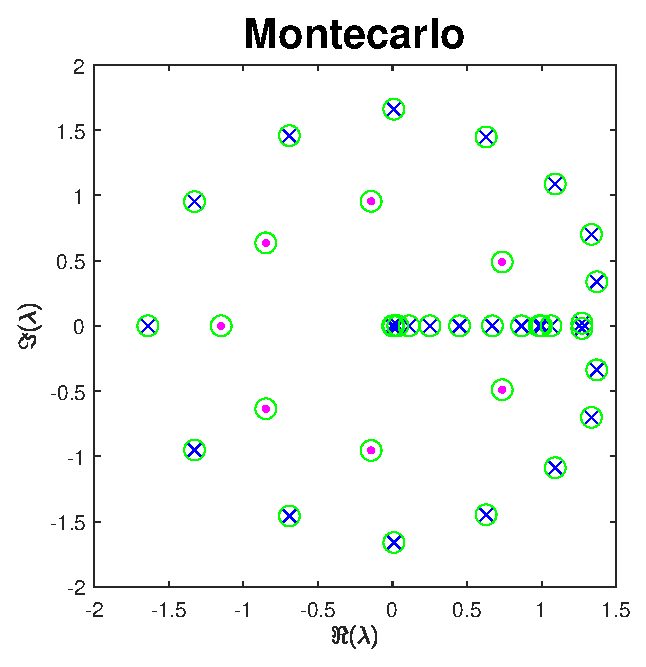
\includegraphics[width=0.25\linewidth]{../code/figures/gauss_map/ResDMD_Montecarlo.eps}
    \hspace*{\fill}
    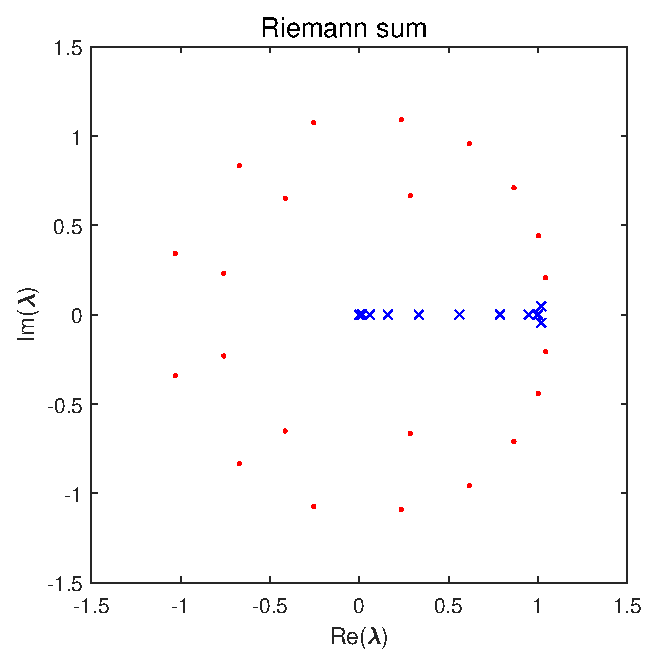
\includegraphics[width=0.25\linewidth]{../code/figures/gauss_map/ResDMD_Riemann.eps}
    \hspace*{\fill}
    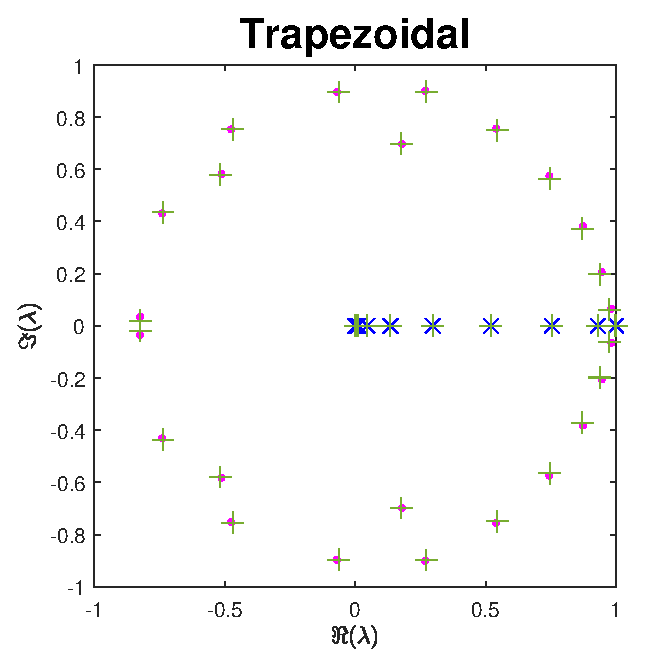
\includegraphics[width=0.25\linewidth]{../code/figures/gauss_map/ResDMD_Trapezoidal.eps}
    \hspace*{\fill}
    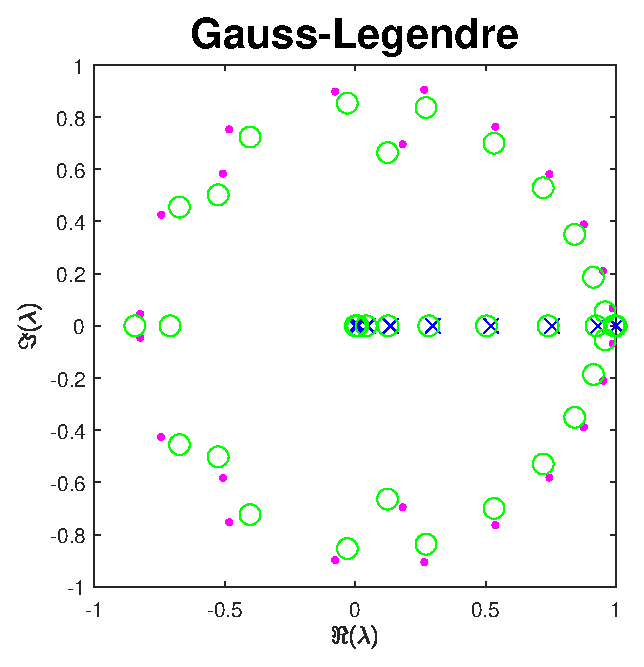
\includegraphics[width=0.25\linewidth]{../code/figures/gauss_map/ResDMD_Gauss-Legendre.eps}
    \hspace*{\fill}
}
\caption{Approximations of the eigenvalues of the Koopman Operator associated with the Gauss iterated map computed with the DMD algorithm (green circles) and the EDMD algorithm (magenta dots and blue crosses), using different quadrature rules. The approximate eigenvalues are computed using $K=40$ observables and $M = 100$ quadrature points. The blue crosses indicate the eigenvalues retained by ResDMD, with tolerance $\varepsilon = 0.01$.}
\label{fig_resdmd_quadrature_comparison}
\end{figure}

\begin{figure}[h]
\makebox[\textwidth][c]{
    \begin{subfigure}{0.45\textwidth}
        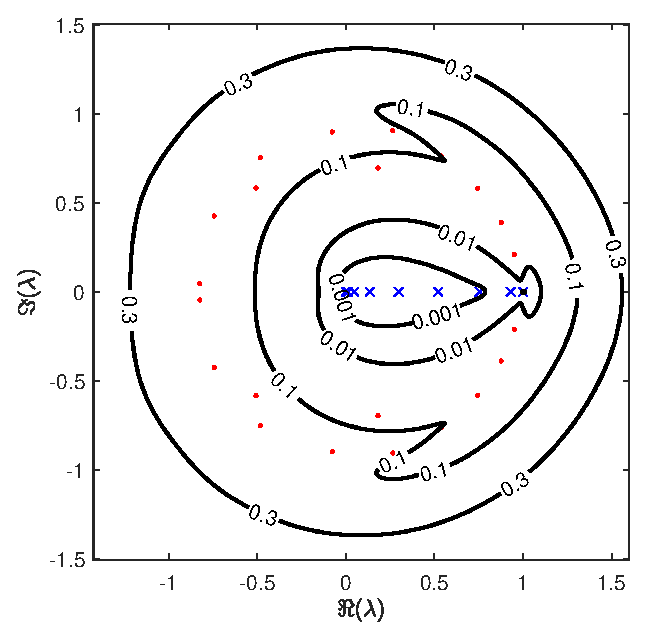
\includegraphics[width=\linewidth]{../code/figures/gauss_map/pseudospectra_contour.eps}
        \caption{Pseudospectral contours}
        \label{gauss_contours}
    \end{subfigure}\hspace*{\fill}
    \begin{subfigure}{0.45\textwidth}
        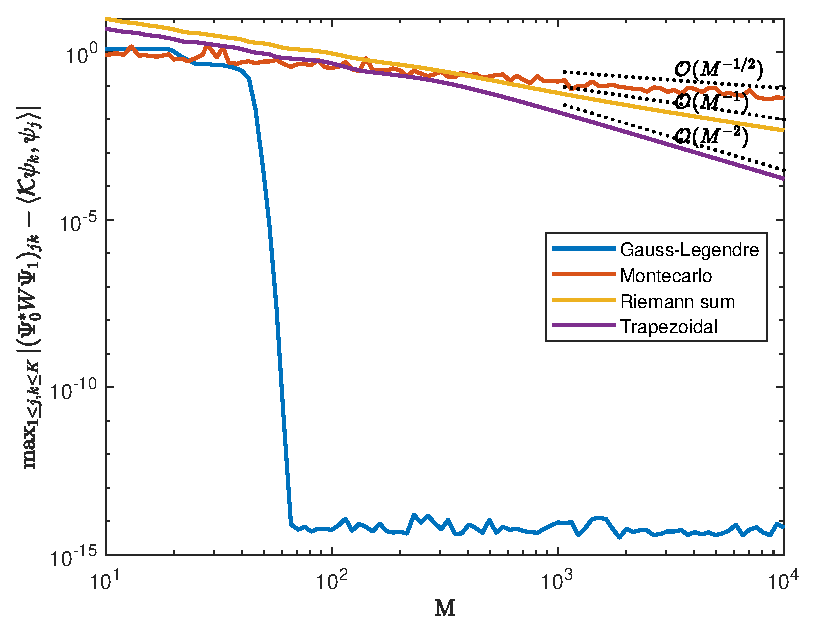
\includegraphics[width=\linewidth]{../code/figures/gauss_map/Galerkin_convergence.eps}
        \caption{Convergence of the quadrature rules}
        \label{gauss_convergence}
    \end{subfigure}\hspace*{\fill}
    }
    \caption{Contour lines of the $\varepsilon$-pseudospectrum for $\varepsilon = 0.3,\,0.1,\,0.01,\,0.001$ computed using \Cref{alg_pseudospectrum} with dictionary of $K=40$ observables (\Cref{gauss_contours}) and convergence of one of the approximate integrals for the different quadrature rules measured as $\max_{1\leq j,k \leq K} \abs{(\Psi_0^* W \Psi_1)_{jk} - \langle\mathcal{K}\psi_k, \psi_j\rangle}$ (\Cref{gauss_convergence}).}
    \label{gauss_pseudospectrum_convergence}
\end{figure}

\subsection{Nonlinear pendulum}
Let us consider the continous-time dynamical system of the nonlinear pendulum. The state variable is $\vb{x} = (x_1, x_2) = (\theta, \dot{\theta}) \in \Omega = [-\pi, \pi]_{\text{per}} \times \R$ and the differential equation governing the motion is
\begin{equation}
    \label{pendulum_equation}
    \dot{\vb{x}} = 
    \begin{bmatrix}
    \dot{x}_1 \\
    \dot{x}_2
    \end{bmatrix} = 
    \begin{bmatrix}
    x_2 \\
    -\sin(x_1)
    \end{bmatrix}.
\end{equation}
We consider the corresponding discrete-time dynamical system with time-step $\Delta_t = 0.5$ and the associated Koopman Operator. The system is Hamiltonian and hence the Koopman Operator is unitary \cite{koopman_hamiltonian_1931}.

The choice of the dictionary of observables is now more complex, because the function governing the motion is vector-valued (with two components) and periodic in the first component. Since the motion is periodic in $x_1\in[-\pi,\pi]_{\text{per}}$, it is natural to use the Fourier basis $\{e_n\}_{n\in\mathbb{Z}}$ in $x_1$ to describe the motion in this direction. Similarly, to approximate the motion in the direction of $x_2$ one might decide to use the Hermite functions $\{h_n\}_{n\in\mathbb{N}}$, which form a basis of the Hilbert space $L^2(\R)$. Therefore, we would ideally consider observables of the form $\phi(x_1, x_2) = \sum_{n\in\mathbb{Z},\,m\in\mathbb{N}} \alpha_{n,m} e_n(x_1)\cdot h_m(x_2)$ for some coefficients $\{\alpha_{n,m}\}\in\C$. However, our dictionary of observables must be finite and we need to decide a criterion to truncate the sum. Observe that there isn't a natural ordering as if the indices were in $\mathbb{N}$ or $\mathbb{Z}$. Since we want to be able to approximate the (components of the) full state observable, it is important to have the indices $\{(n,0)\}_{n=0}^{n_{\max}}$ and $\{(0,m)\}_{m=-m_{\max}}^{m_{\max}}$ with $n_{\max},\,m_{\max}$ as high as possible. Selecting the indices in the rectangle $\{(n,m)\,:\,-n_{\max}\leq n\leq n_{\max},\,\, 0\leq m\leq m_{\max}\}$ would make the size of the dictionary grow too fast in $n_{\max}$ and $m_{\max}$, thus we use an hyperbolic cross approximation \cite{dung_hyperbolic_2017}, i.e. we select the indices in the hyperbolic cross $\{(n,m)\,:\, \max(n,1)\cdot \max(m,1)\leq N \}$, where $N$ is called the order of the hyperbolic cross approximation.

Using \Cref{alg_pseudospectrum} we compute an approximation of the $\varepsilon$-pseudospectrum for $\varepsilon = 0.25$, first using $K=193$ observables and $M = 10^4$ data points, then employing $K=1265$ and $M = 9 \times 10^4$. As the size $K$ of the dictionary increases, the approximation of the $\varepsilon$-pseudospectrum approaches the annulus with internal radius 0.75 and external radius 1.25(see \Cref{pendulum_pseudospectrum}). We also compute approximation of the eigenfunctions associated with the eigenvalues $\lambda = \exp(0.4932 i), \,\lambda = \exp(0.9765 i), \,\lambda = \exp(1.4452 i), \,\lambda = \exp(1.8951 i), \,$ (see \Cref{pendulum_phase_portraits}).

\begin{figure}[h]
\makebox[\textwidth][c]{
    \begin{subfigure}{0.45\textwidth}
        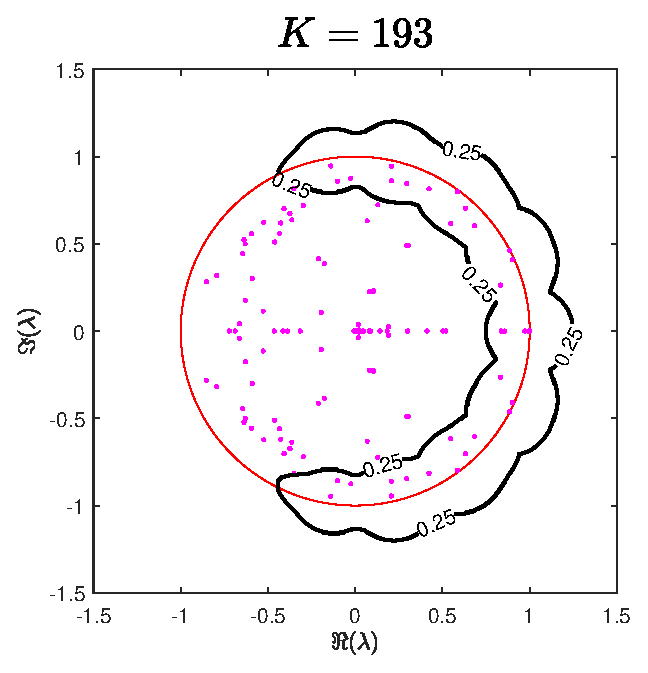
\includegraphics[width=\linewidth]{../code/figures/pendulum/pendulum_N193.eps}
    \end{subfigure}\hspace*{\fill}
    \begin{subfigure}{0.45\textwidth}
        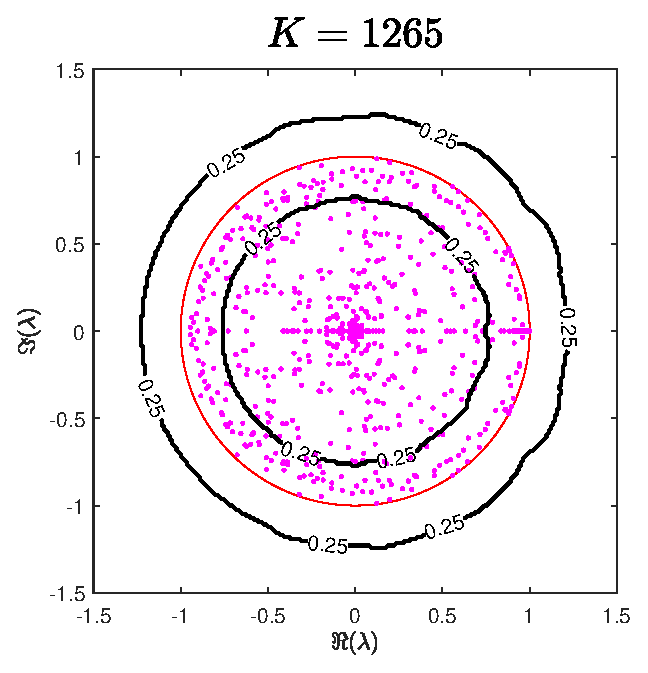
\includegraphics[width=\linewidth]{../code/figures/pendulum/pendulum_N1265.eps}
    \end{subfigure}\hspace*{\fill}
        }
    \caption{Contour lines of the $\varepsilon$-pseudospectrum for $\varepsilon = 0.25$ computed using \Cref{alg_pseudospectrum} with hyperbolic cross approximation. On the left the approximation obtained using a dictionary of $K=193$ observables and $M = 10^4$ data points, on the right the one obtained with $K=1265$ and $M = 9 \times 10^4$.}
    \label{pendulum_pseudospectrum}
\end{figure}

\begin{figure}[h]
\centering
\makebox[\textwidth][c]{
        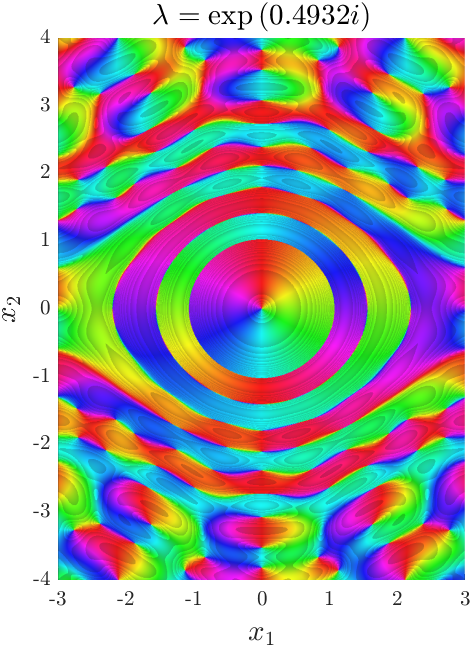
\includegraphics[width=0.25\linewidth]{../code/figures/pendulum/phase_portrait_4932.png}
        \hspace*{\fill}
        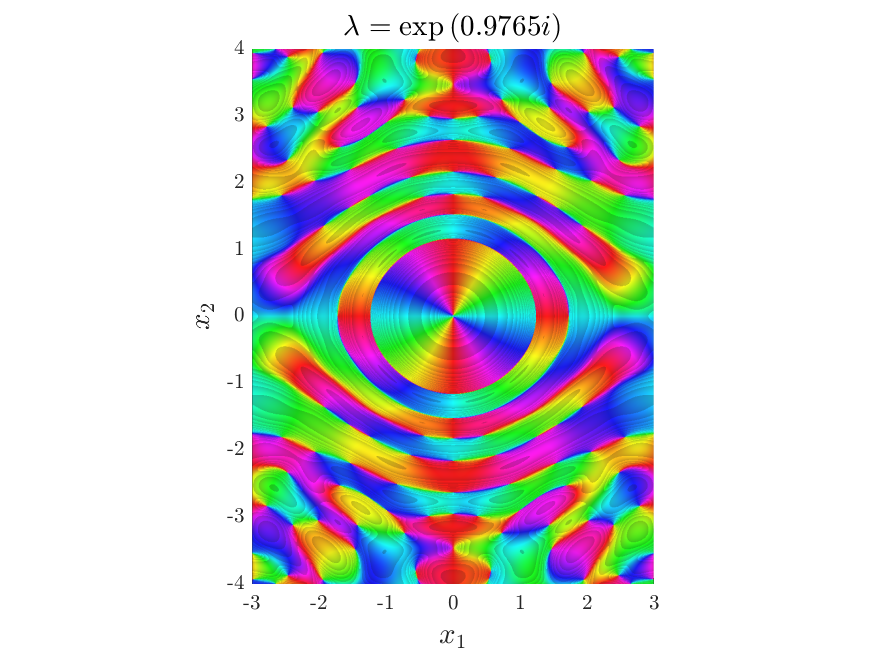
\includegraphics[width=0.25\linewidth]{../code/figures/pendulum/phase_portrait_9765.png}
        \hspace*{\fill}
        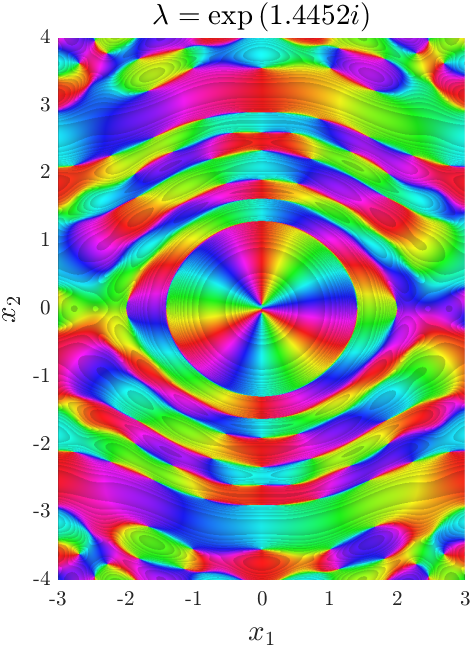
\includegraphics[width=0.25\linewidth]{../code/figures/pendulum/phase_portrait_14452.png}
        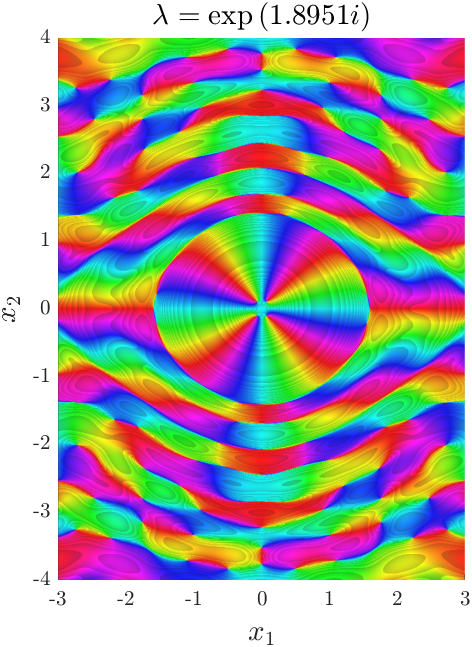
\includegraphics[width=0.25\linewidth]{../code/figures/pendulum/phase_portrait_18951.png}
        \hspace*{\fill}}
        \caption{Phase portraits of the approximate eigenfunctions of the nonlinear pendulum, where the color illustrates the complex argument of the eigenfunction. Lines of constant modulus are plotted as shadowed steps.}
        \label{pendulum_phase_portraits}
\end{figure}
